\documentclass[11pt,a4paper]{article}

% =========================================================
% EASY CONTROLS
% Change only these first when you want to tune the layout.
% =========================================================
\usepackage[
    a4paper,
    top=1.0in,
    bottom=1.0in,
    left=1.02in,
    right=1.02in
]{geometry} 

\newcommand{\TitleFont}{\fontsize{15.5}{17.5}\selectfont}
\newcommand{\AuthorFont}{\normalsize}
\newcommand{\AffilFont}{\small}
\newcommand{\AbstractFont}{\small}
\renewcommand{\baselinestretch}{1.04} 

% =========================================================
% PACKAGES
% =========================================================
\usepackage[T1]{fontenc}
\usepackage[utf8]{inputenc}
\usepackage{newtxtext,newtxmath} 
\usepackage{microtype}           
\usepackage{graphicx}
\usepackage{booktabs}
\usepackage{array}
\usepackage{enumitem}
\usepackage{hyperref}
\usepackage{titlesec}
\usepackage{caption}
\usepackage{setspace}
\usepackage{xcolor}
\usepackage{placeins} % Added to prevent figures from floating into references

% =========================================================
% GENERAL FORMATTING
% =========================================================
\hypersetup{
    colorlinks=true,
    linkcolor=blue,
    urlcolor=blue,
    citecolor=blue
}

\setlength{\parindent}{1.2em}
\setlength{\parskip}{0pt}
\setlength{\emergencystretch}{1.5em} 

\titleformat{\section}{\large\bfseries}{\thesection}{0.7em}{}
\titleformat{\subsection}{\normalsize\bfseries}{\thesubsection}{0.7em}{}
\titlespacing*{\section}{0pt}{1.4ex plus 0.4ex minus 0.2ex}{0.7ex}
\titlespacing*{\subsection}{0pt}{1.0ex plus 0.3ex minus 0.2ex}{0.5ex}

\captionsetup{
    font=small,
    labelfont=bf
}

\setlist[itemize]{
    leftmargin=1.4em,
    itemsep=0.15em,
    topsep=0.25em
}

\setlist[enumerate]{
    leftmargin=1.6em,
    itemsep=0.15em,
    topsep=0.25em
}

% =========================================================
% TITLE
% =========================================================
\title{}
\author{}
\date{}

\begin{document}

\begin{center}
{\TitleFont\bfseries
DBSHIELD: DataBase Systems Handling for Injection, Exploitation, Leakage, and DoS
\par}

\vspace{0.65em}

{\small
\begin{tabular}{c}
Arnav Priyadarshi (23CS30008) \quad
Ketan Suman (23CS30027) \quad
Krishna Prabu (23CS30028) \\[0.25em]
Rahul Chandrakant Patne (23CS10084) \quad
Shreeraj Kalbande (23CS30025) \\[0.35em]
\end{tabular}
\par}

\vspace{0.7em}
\end{center}

\section{Problem Statement}

Modern web applications depend heavily on databases to store and process sensitive information such as credentials, personal records, academic data, and administrative entries. Thus, it is important to study and understand how to construct secure databases. Ignoring this often leads to insecure design decisions such as unsafe query construction, weak validation of user-controlled input, insufficient server-side access checks, and inadequate controls against computational abuse. When such weaknesses exist in a database-backed system, the consequences can include unauthorized access, leakage of sensitive information, loss of service availability and more.

We present the \textbf{DBSHIELD} project, motivated by the need to demonstrate that these issues are not merely theoretical, but can arise in many places during development. Many users and developers underestimate how severely a database system can be affected when core security mechanisms are absent or improperly implemented. Instead of discussing these risks only in abstract terms, we aim to present through this project a direct comparison between two versions of the same application: an \textit{unshielded} system that is intentionally vulnerable for controlled demonstration, and a \textit{shielded} system that includes appropriate safeguards. This side-by-side design makes the role of security measures obvious, and shows how without them the system can be significantly harmed.

The application selected for this project is a mock student ERP system with three roles: \textit{student}, \textit{teacher}, and \textit{admin}. We selected this setting as it is something the intended audience can relate to easily, and reflects a realistic role-based application in which users authenticate, access restricted information, perform role-specific actions, and interact with shared database records. Such a system will naturally expose the central security requirements of authentication, data isolation and resilience. It therefore provides a practical environment in which database related vulnerabilities and their mitigations can be examined in a meaningful way.

We focus on three representative classes of attack. The first is \textit{SQL injection}, which targets the interaction between user input and backend query execution. When queries are not handled safely, SQL injection may allow login bypass, unauthorized reads, and unintended modifications to database contents. The second is \textit{denial of service}, studied here in the form of expensive application or database requests that can degrade responsiveness or exhaust resources. The third is \textit{authorization bypass}, where a user attempts to access resources or operations outside the limits of their intended role, particularly in systems that trust client-side verification such as cookies over server-side verification.

\section{Methodology}

\subsection{Overall Study Design}

Two functionally similar versions of the same student ERP application are designed and studied:

\begin{itemize}
    \item \textbf{Unshielded system:} A deliberately vulnerable implementation in which protections are absent, to demonstrate the importance of defending against attacks.
    \item \textbf{Shielded system:} A hardened implementation that preserves the same functionality while incorporating defensive mechanisms to prevent attacks.
\end{itemize}

This paired design helps isolate the effect of security controls. Since both systems serve the same use case and operate on the same general model of data and user roles, differences in observed behavior can be attributed more clearly to the presence or absence of safeguards rather than to unrelated architectural changes.

\subsection{System Under Study}

The application modeled in this project is a student ERP system with three user roles:

\begin{itemize}
    \item \textbf{Student:} Accesses personal details, academic information, and self-related records. Can enroll in courses, deregister from courses, but not view or interact with other students.
    \item \textbf{Teacher:} Accesses and updates academic information related to students and courses. Can create courses, modify contents, but cannot modify other teacher's courses.
    \item \textbf{Admin:} manages users, records, and privileged system-level operations.
\end{itemize}

This role structure is intentionally chosen because it captures a realistic multi-user scenario in which different permissions must be enforced over the same database. It provides a suitable basis for studying authentication flows, role-based restrictions, protected data access, and misuse of sensitive operations.

\subsection{Technology Stack}

The system uses a web-application stack composed of the following components:

\begin{itemize}
    \item \textbf{Frontend:} React is used to build the user-facing interface, including login pages, dashboards, navigation, and role-specific views.
    \item \textbf{Backend:} FastAPI is used to implement API endpoints, application logic, authentication handling, request processing, and access control logic.
    \item \textbf{Database:} PostgreSQL and SQLite is used as the relational data store for user accounts, role information, academic records, and related entities.
\end{itemize}

\subsection{Unshielded and Shielded Implementations}

In both the cases, the FastAPI backend is responsible for retrieving from the database, perform logical operations, checking and communicating the result to the frontend.

In the \textit{Unshielded Implementation}, the raw SQL is directly fed, without any additional checking, to the database to fetch data. This can cause issues such as SQL Injection, DoS and Authorization Bypass, which are discussed later. The result similarly is directly fed to the user, without verification.

In the \textit{Shielded Implementation}, the input from the frontend is processed, checked for potential SQL Injection attacks, checked for DoS attacks, and is only then processed. This avoids issues that used to arise in the unshielded implementation.

\subsection{Evaluation Criteria}

For each attack category, the final comparison between the unshielded and shielded systems is organized using the following criteria:

\begin{itemize}
    \item \textbf{Attack success:} whether the intended misuse achieves its goal.
    \item \textbf{Impact scope:} what data, role, or service is affected.
    \item \textbf{Response behavior:} whether the system leaks information, hangs, returns unsafe errors, or fails in a controlled way.
    \item \textbf{Resilience:} whether the application remains stable and recoverable during and after testing.
    \item \textbf{Mitigation effectiveness:} whether the shielded system prevents or significantly limits the observed issue.
\end{itemize}

% =========================================================
% SYSTEM ARCHITECTURE
% =========================================================
\section{System Architecture}

The system architecture is structured as a modern, decoupled web application. The frontend is built utilizing React, providing a dynamic single-page application (SPA) experience. State management is handled through a combination of React Context and custom hooks, ensuring that user session data and role information persist across component re-renders. Routing is managed securely on the client side to restrict navigation to unauthorized views based on the logged-in user's role. However, as demonstrated in our authorization bypass studies, client-side routing is fundamentally insufficient for actual security, placing the burden of enforcement entirely on the backend architecture.

The backend is engineered using FastAPI, a modern, high-performance web framework for building APIs with Python. We leverage FastAPI's powerful dependency injection system to handle routing logic, database session management, and the crucial \texttt{ENABLE\_SQLI\_PROTECTION} toggle. In the application code, endpoints accept an injected database session parameter. When the protection toggle is set to false, the dependency yields a raw database cursor capable of executing unparameterized string concatenations. When true, the dependency strictly yields an Object-Relational Mapping (ORM) session or enforces parameterized query building, fundamentally changing the data access layer's behavior without requiring code changes within the individual endpoint functions.

The database layer utilizes a dual-engine setup consisting of PostgreSQL and SQLite to demonstrate vulnerability persistence across different SQL dialects. The core schema is normalized and consists of several key tables: a \texttt{Users} table storing authentication credentials and a foreign key linking to a \texttt{Roles} table; a \texttt{Courses} table detailing available curriculum offerings; an \texttt{Enrollments} table acting as a junction linking students to courses; and a \texttt{Grades} table. By structuring the database with explicit foreign key constraints and distinct data silos, we ensure that our authorization bypass and data leakage tests have clearly defined boundaries to violate in the unshielded system and protect in the shielded system.

\begin{figure}[h!]
    \centering
    \framebox(400, 200){[PLACEHOLDER: High-Level System Architecture Diagram]}
    \caption{High-level overview of the DBSHIELD system architecture.}
    \label{fig:architecture}
\end{figure}

\begin{figure}[h!]
    \centering
    \framebox(400, 200){[PLACEHOLDER: Database Entity-Relationship (ER) Diagram]}
    \caption{Entity-Relationship diagram mapping users, roles, and academic records.}
    \label{fig:er_diagram}
\end{figure}

\section{SQL Injection}

\subsection{Study}

The SQL injection study now covers both authentication and several ERP data-handling endpoints. The backend preserves an intentionally vulnerable implementation in its original service layer, while the hardened behavior is implemented in a separate module under \texttt{sql\_injection\_prevention}. A single runtime flag, \texttt{ENABLE\_SQLI\_PROTECTION}, determines which handler is used for each request. This paired design is useful for controlled evaluation because the application routes, payload formats, and user-visible functionality remain unchanged, while only the query-construction strategy differs between the two modes.

In the unshielded mode, multiple operations continue to build SQL directly from user-controlled values. These include login, course search, grade and course lookups based on usernames, enrollment and grading workflows, administrative creation and deletion actions, and an especially sensitive admin query endpoint. In the shielded mode, the same operations are routed to secure counterparts that use parameterized queries for user-supplied values. For the admin query interface, which accepts free-form SQL text by design, the secure path does not attempt to parameterize arbitrary statements; instead, it restricts execution to a single read-only \texttt{SELECT} or \texttt{WITH} query and blocks mutating or stacked statements.

To evaluate this design, we use a controlled set of payloads against both the login path and representative ERP endpoints. The test corpus includes authentication-bypass inputs based on comments and tautologies, \texttt{UNION}-style payloads intended to forge result rows or enumerate schema information, and username or course-code payloads intended to alter selection or deletion behavior in routine ERP operations. Additional tests also check whether values that look like SQL fragments, such as a malicious-looking grade string or username, are stored and handled as literal data in the secure mode rather than being executed as part of the query.

The experiments are executed through the project test harness and through the application toggle that switches between vulnerable and secure handlers. For each case, the main observation is whether the supplied payload changes query semantics, broadens the result set, causes unintended data modification, or bypasses the intended restriction on the admin action endpoint. The comparison therefore measures not only whether login injection is prevented, but also whether the same defensive strategy generalizes across the broader ERP workflow.

\subsection{Results}

The updated SQL injection experiments show a consistent separation between the vulnerable ERP service layer and the shielded handlers selected through \texttt{ENABLE\_SQLI\_PROTECTION}. On the login path, the previously documented SQLite-compatible payloads continued to succeed against the unshielded implementation: comment-based and tautology payloads enabled authentication bypass, \texttt{UNION}-based payloads could fabricate or expose rows, and blind inference payloads could still alter query logic. This confirms that the vulnerable path remains suitable for controlled demonstration.

The broader ERP tests show the same pattern. In the unshielded mode, username-based injection payloads could broaden student-grade and student-course lookups, and course-search input could alter selection behavior. Administrative actions that interpolate course codes or usernames are likewise exposed in the vulnerable path because the query text is still assembled directly from request data. In contrast, the shielded handlers treat these same payloads as literal values. Search and lookup functions return no unauthorized data, delete operations do not affect unintended rows, enrollment requests using injected usernames fail normally, and malicious-looking values can be stored as plain data without changing query structure.

\begin{figure}[h!]
    \centering
    \framebox(400, 200){[PLACEHOLDER: Screenshot of Successful Unshielded SQLi Bypass]}
    \caption{Successful login bypass in the unshielded implementation using a tautology payload.}
    \label{fig:sqli_unshielded}
\end{figure}

\begin{figure}[h!]
    \centering
    \framebox(400, 200){[PLACEHOLDER: Screenshot of Shielded System Blocking SQLi]}
    \caption{Shielded system securely treating the malicious payload as a literal string.}
    \label{fig:sqli_shielded}
\end{figure}

The hardened admin action endpoint is a particularly important result. Since this interface is meant to accept SQL text, parameterization alone is not sufficient. The secure implementation therefore adds a structural restriction: only a single read-only \texttt{SELECT} or \texttt{WITH} statement is accepted. As a result, mutating statements such as \texttt{DROP TABLE}, \texttt{UPDATE}, or stacked multi-statement payloads are rejected, while legitimate read-only queries continue to work. This makes the defense more realistic for a free-form admin query feature, where the goal is controlled capability rather than complete removal of functionality.

\begin{table}[h]
\centering
\caption{Observed outcome of SQL injection tests after adding toggle-based secure handlers}
\begin{tabular}{p{0.31\linewidth} p{0.28\linewidth} p{0.28\linewidth}}
\toprule
\textbf{Payload category} & \textbf{Unshielded system} & \textbf{Shielded system} \\
\midrule
Comment and tautology login bypass & Successful unauthorized login & Blocked; login fails normally \\
\texttt{UNION}-based data extraction & User data and query-controlled rows returned & Blocked; no data disclosure \\
\texttt{UNION}-based role forgery and schema manipulation & Forged or metadata-oriented rows can be returned & Blocked; payload treated as data \\
Injected usernames in student lookups & Result set can be broadened beyond intended user & Blocked; no unauthorized rows returned \\
Injected course codes in admin delete/search paths & Query behavior can be altered & Payload treated literally; intended row scope preserved \\
Injected values in enroll/grade/create operations & May alter query semantics in vulnerable flow & Stored or rejected as plain data without execution \\
Mutating or stacked admin SQL & Can execute directly on vulnerable path & Rejected unless it is a single read-only query \\
\bottomrule
\end{tabular}
\end{table}

Some additional payloads were also examined to clarify the limits of the current demonstration. PostgreSQL-specific constructs such as \texttt{pg\_sleep()}, \texttt{version()}, or \texttt{information\_schema}-based extraction did not succeed against the current vulnerable login path because the project uses SQLite for this experiment. Similarly, a stacked-query payload attempting to append an \texttt{INSERT} statement raised an execution error rather than succeeding, because the present \texttt{sqlite3.execute()} path does not permit multiple statements in that form. These cases are important because they show that not every SQL injection string is universally portable; however, they do not weaken the main result. The vulnerable system remains exploitable by several practical SQLite-compatible payloads, whereas the shielded system prevents the tested SQL injection attempts while preserving normal authentication behavior.

\section{Denial of Service}

\subsection{Study}

The denial-of-service study focuses on the ERP login endpoint, because this path is intentionally expensive in the vulnerable configuration and therefore makes the effect of attack traffic easy to observe. For this demonstration, the SQL-injection toggle is kept disabled so that \texttt{/api/login} uses the vulnerable \texttt{handle\_student\_login()} path, which includes an artificial delay before the database query. In the unshielded setting, \texttt{ENABLE\_DDOS\_PROTECTION = False}, so all login requests, including attacker traffic with invalid credentials, are allowed to reach this delayed path. As a result, repeated login floods consume worker capacity and make the frontend noticeably less responsive for legitimate users.

The shielded setting keeps the same endpoint and frontend behavior, but enables the DDoS wrapper around the application. The attack script repeatedly submits randomized login attempts and attaches spoofed \texttt{X-Forwarded-For} headers. In the current local deployment, the middleware treats such client-supplied forwarded headers as untrusted and rejects those requests before the expensive login code runs. Legitimate browser traffic does not carry this header and therefore continues normally. The shielded login path also uses a bounded semaphore around expensive authentication work, which prevents bursts from creating unbounded concurrent load. The purpose of the comparison is therefore to show that the unshielded system allows attack traffic to consume the costly login path, whereas the shielded system blocks spoofed traffic early enough to preserve normal responsiveness.

\paragraph{Demonstration setup.}
The demonstration can be reproduced locally by launching the backend, frontend, and attack script from their respective directories:
\begin{quote}
\small\ttfamily
cd backend \\
uvicorn app:app --host 127.0.0.1 --port 8000 \\[0.3em]
cd frontend/frontend \\
npm start \\[0.3em]
cd ddos\_attack \\
python3 ddos\_simulator.py
\end{quote}
With \texttt{ENABLE\_DDOS\_PROTECTION = False}, the attacker traffic reaches the delayed login path and the frontend becomes visibly slower during the flood. With \texttt{ENABLE\_DDOS\_PROTECTION = True}, the same spoofed attack requests are rejected in middleware and should no longer reach the expensive login handler; the expected observation is that ordinary frontend interaction remains much smoother even while the attack script is running.

\subsection{Results}

The implemented defense produces a clear qualitative separation between the vulnerable and shielded modes. In the unshielded run, attacker requests are still processed by the delayed login path and therefore consume time even though they eventually fail authentication. Under sustained flooding, this makes the login experience slower for a real user operating through the frontend. In the shielded run, the spoofed requests are rejected before the delayed login handler is reached, so the backend avoids spending that artificial database cost on attacker traffic.

This difference is consistent with the present implementation. The attacker script deliberately sends \texttt{X-Forwarded-For} headers, while the local middleware rejects such headers as untrusted. Consequently, in the shielded configuration the dominant attacker-facing outcome is early rejection, and the normal browser path remains separated from the spoofed flood. The protection is therefore not merely reducing the number of successful logins by the attacker; it is preserving availability by preventing malicious requests from reaching the expensive part of the authentication flow.
\renewcommand{\arraystretch}{1.5}
\begin{table}[h]
\centering
\small
\caption{Observed qualitative behavior of the DoS demonstration.}
\label{tab:dos_results}
\begin{tabular}{%
    >{\raggedright\arraybackslash}p{0.26\linewidth}
    >{\raggedright\arraybackslash}p{0.21\linewidth}
    >{\raggedright\arraybackslash}p{0.20\linewidth}
    >{\raggedright\arraybackslash}p{0.22\linewidth}}
\toprule
\textbf{Mode} & \textbf{Attacker request path} & \textbf{Typical attacker outcome} & \textbf{Observed user experience} \\
\midrule
Unshielded
(\texttt{ENABLE\_DDOS\_PROTECTION\allowbreak\ =\ False})
    & Requests reach the delayed login handler
    & Authentication fails only after backend work is spent
    & Frontend becomes noticeably slower under sustained attack \\[0.4em]
Shielded
(\texttt{ENABLE\_DDOS\_PROTECTION\allowbreak\ =\ True})
    & Spoofed requests are blocked in middleware before login execution
    & Early rejection, typically HTTP~403
    & Frontend remains substantially more responsive during the same attack \\
\bottomrule
\end{tabular}
\end{table}

\section{Authorization Bypass}

\subsection{Study}

The third attack category studies authorization bypass. Because the ERP has clearly separated user roles, it is important to evaluate whether a user can access functions or records beyond their intended permissions. This includes scenarios such as requesting pages intended for another role, directly invoking restricted backend endpoints, or attempting to retrieve or modify records that should not be accessible under the current identity.

In this part of the project, the backend first performs authentication and then demonstrates the separate question of authorization. After a successful login, the server generates a fresh random bearer token and stores it in an in-memory token table that maps the token to the authenticated user's \texttt{username} and \texttt{role}. Subsequent requests are therefore not allowed to declare their role directly through client-controlled headers; instead, the backend extracts the bearer token, looks it up on the server, and recovers the associated identity and role from that mapping. This design is useful in the report because it makes the distinction between ``logged in'' and ``allowed to do this action'' very explicit.

The unshielded and shielded versions differ in what happens \emph{after} token verification. In both cases, a request must still present a valid token that was issued at login time. In the unshielded mode, selected endpoints intentionally skip the role and ownership checks once the token is accepted, which allows a valid student session to invoke instructor or admin operations or to request another student's records. In the shielded mode, the same token-derived role is checked on the server for every protected endpoint, and student-facing data lookups also verify ownership where required. A runtime flag, \texttt{ENABLE\_AUTH\_BYPASS\_PROTECTION}, switches between these two behaviors without changing the external API.

This comparison highlights the core lesson of the authorization-bypass study: authentication alone is not sufficient. Even when a token correctly represents a real logged-in user, the backend must still verify that the role attached to that token is permitted to perform the requested action and, where necessary, that the requested data belongs to that user.

\paragraph{Testing procedure.}
For controlled testing, the variable \texttt{ENABLE\_AUTH\_BYPASS\_PROTECTION} in the backend is switched between \texttt{False} (unshielded authorization behavior) and \texttt{True} (shielded authorization behavior). A typical test first logs in as a student to obtain a bearer token and then reuses that token against an endpoint that should require a stronger role. For example:

\begin{quote}
\small\ttfamily
TOKEN=\$(curl -s -X POST http://localhost:8000/api/login \textbackslash{}\\
\hspace*{1.6em}-H "Content-Type: application/json" \textbackslash{}\\
\hspace*{1.6em}-d '\{"username":"student1","password":"pass1"\}' | jq -r '.token')
\end{quote}

The expected outcome of this login request is a successful response containing a token together with the authenticated \texttt{username} and \texttt{role}. That token can then be used to test a protected admin endpoint:

\begin{quote}
\small\ttfamily
curl -s -X POST http://localhost:8000/api/admin/action \textbackslash{}\\
\hspace*{1.6em}-H "Authorization: Bearer \$TOKEN" \textbackslash{}\\
\hspace*{1.6em}-H "Content-Type: application/json" \textbackslash{}\\
\hspace*{1.6em}-d '\{"query":"SELECT username FROM users LIMIT 1"\}' | jq .
\end{quote}

When \texttt{ENABLE\_AUTH\_BYPASS\_PROTECTION = False}, the expected output is a successful response such as \texttt{\{"message":"Admin action executed.", ...\}}, even though the token belongs to a student. When \texttt{ENABLE\_AUTH\_BYPASS\_PROTECTION = True}, the same request is expected to fail with a controlled authorization error such as HTTP 403 and an \texttt{Access denied} message. A second useful test is to call \texttt{/api/student/view-grades} with another student's username while logged in as \texttt{student1}; the vulnerable mode returns another student's data, whereas the shielded mode returns a denial based on ownership checking.

\subsection{Results}

The authorization-bypass experiments showed a clear separation between authentication and authorization in the implemented backend. A user could obtain a bearer token only after a successful login at \texttt{/api/login}, and the server stored that token in its in-memory token table together with the corresponding \texttt{username} and \texttt{role}. Later requests therefore used a real authenticated session; the bypass behavior did not come from forged headers or fake identities, but from whether the backend performed role and ownership checks after recovering the session from the token.

In the unshielded mode, the vulnerable behavior remained demonstrable exactly as intended. After logging in as \texttt{student1}, the same student token could be reused to call endpoints such as \texttt{/api/admin/action} or instructor endpoints like \texttt{/api/instructor/assign-grade}, even though those routes are meant for stronger roles. Similarly, a student session could call \texttt{/api/student/view-grades} with another student's username and receive data that should not have been exposed. These outcomes confirmed that the vulnerable configuration represents an authorization failure rather than an authentication failure.

In the shielded mode, the same requests were rejected consistently on the server side. The backend extracted the token, looked it up in the server-side mapping, recovered the user's role, and then compared that role against the allowed roles for the endpoint. Requests to administrator and instructor endpoints from a student token therefore failed with controlled HTTP 403 responses, while cross-user grade access was blocked by the ownership check applied to student data. The main result is therefore that the shielded implementation preserves valid login and session handling while preventing a logged-in user from turning that valid session into unauthorized access.

\begin{figure}[h!]
    \centering
    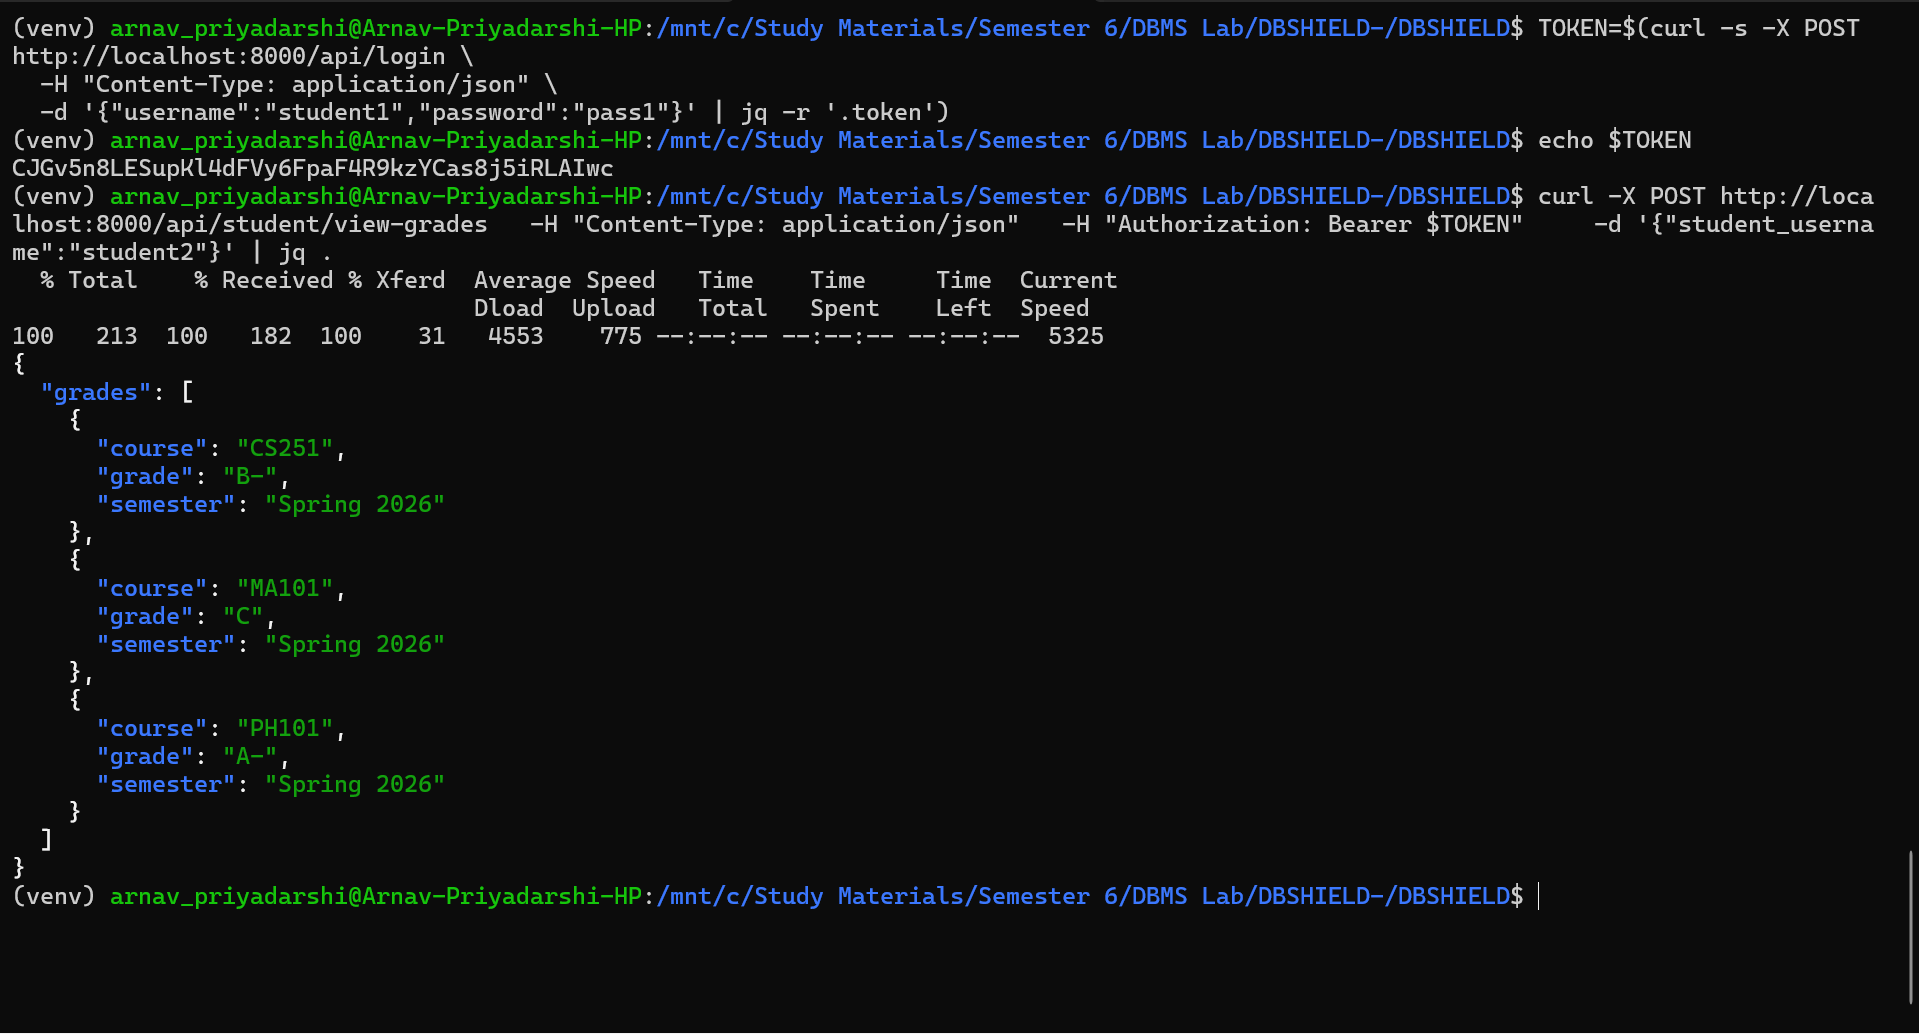
\includegraphics[width=0.8\textwidth]{images/Auth_False.png}
    \caption{Successful authorization bypass in the unshielded implementation.}
    \label{fig:auth_unshielded}
\end{figure}

\begin{figure}[h!]
    \centering
    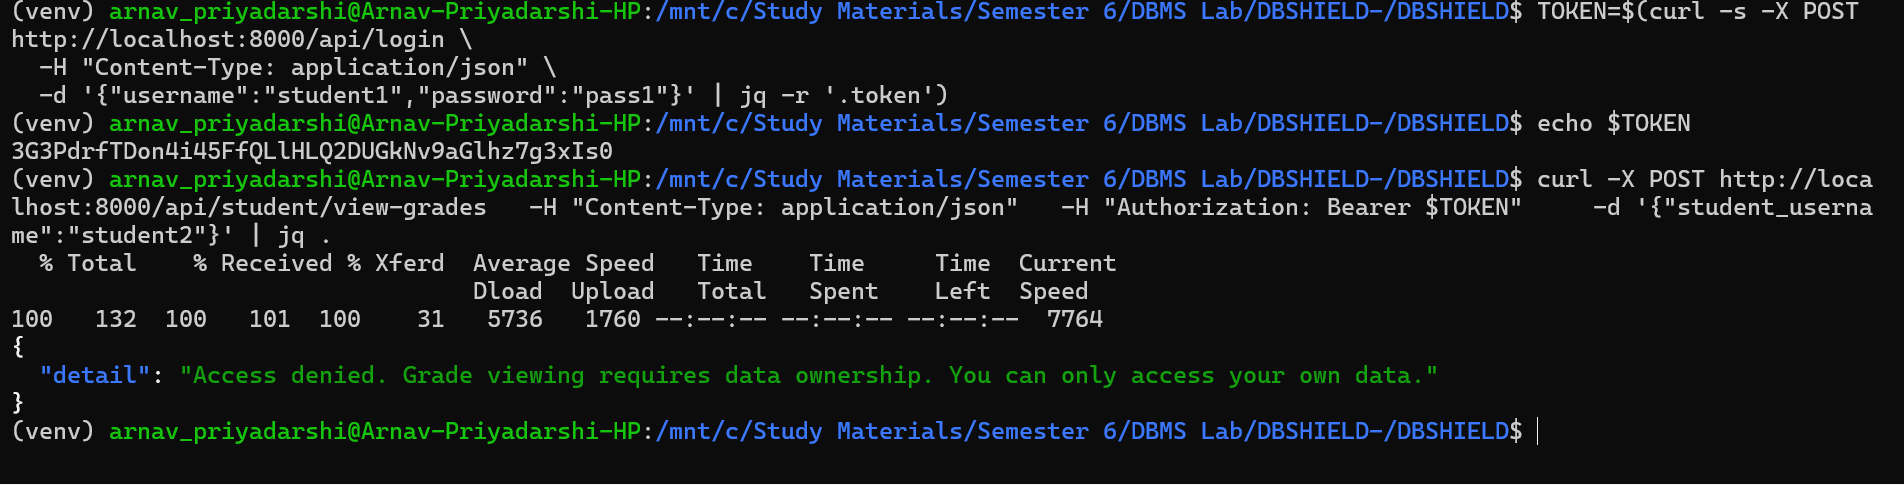
\includegraphics[width=0.8\textwidth]{images/Auth_True.png}
    \caption{Shielded system rejecting the unauthorized request with an HTTP error.}
    \label{fig:auth_shielded}
\end{figure}

% =========================================================
% REFERENCES
% =========================================================
\FloatBarrier % This forces all floating figures above to be printed before starting this section.


\end{document}
